\chapter{Reference}
\label{Reference}
\typeout{$Id$}

\section{Main Window}
\label{Main}

\begin{figure}[hbpt] \begin{centering}
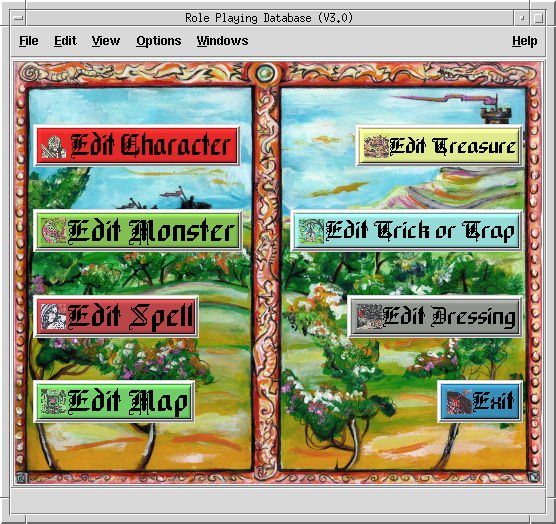
\includegraphics[width=5in]{MainWindow.png} \caption{The main window of
the Role Playing Database} \label{fig:main} \end{centering}
\end{figure} The main window, shown in Figure~\ref{fig:main}, contains
buttons for the seven game informational editors: Character, Monster,
Spell, Treasure, Trick / Trap, Map, and Dressing.  See
Section~\ref{SheetEditor} for a documentation on the Character,
Monster, Spell, Treasure, Trick / Trap, Dressing editor windows and
Section~\ref{Map} for documentation the Map editor window. An eighth
button selects for program exit. In addition to the eight buttons,
there are drop down menus on a menu bar.  The same menu bar is used on
all of the major top level screens.  The File menu has the standard
New, Open, Save, Save As, Print, Close, and Exit menu items, all of
which have the expected meanings and functionality.  The New and Open
menu items on the File menu use cascading menus to select the sort of
thing to create or open.  The Options menu contains menu items to
create/edit (see Section~\ref{sect:configuration}), read, and write the
program's main configuration file, plus a menu item to edit template
files, which opens the ``Sheet Template Editor'' window (See
Section~\ref{Template}), which is used to create and maintain the sheet
editor windows.  The Windows menu contains menu items to select one of
the existing top level windows. The Help menu provides access to the
on line help system (see Chapter~\ref{Help} for complete information
about using the on-line help).

\section{Configuration Editor}
\label{sect:configuration}

\begin{figure}[hbpt]
\begin{centering}
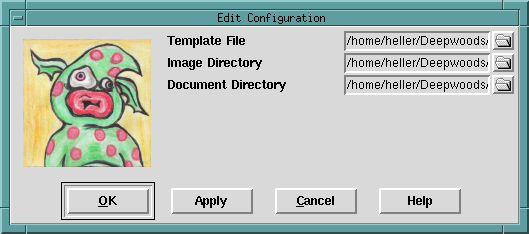
\includegraphics[width=5in]{ConfigurationEditor.png}
\caption{The Configuration Editor Window}
\label{fig:confedit}
\end{centering}
\end{figure}
In Figure~\ref{fig:confedit} is shown the Configuration Editor Window. 
There are three configuration options: the template file to use when
creating new informational sheets, the initial directory to look in for
images for graphic elements, and the initial directory to look in for
external documents.  The configuration file is located in the current
user's home directory in a file named \verb=.roleplayingdb3= under
UNIX/Linux and MacOSX and \verb=roleplayingdb3.rc= under MS-Windows. 
This file is a plain text file containing key, value pairs.  Do not edit
this file by hand though.  Be sure to use the Configuration Editor. 
This makes sure that the file is properly formatted to be read in at
program start time.

\section{Sheet Template Editor Window}
\label{Template}

\begin{figure}[hbpt]
\begin{centering}
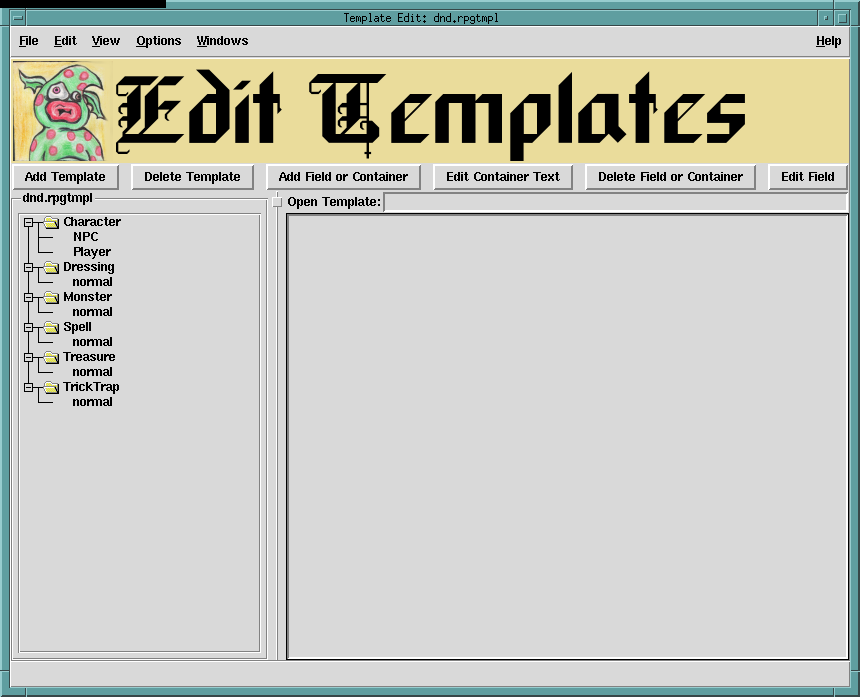
\includegraphics[width=5in]{TemplateEditor1.png}
\caption{The initial Template Editor Window}
\label{fig:tmped1}
\end{centering}
\end{figure}
\begin{figure}[hbpt]
\begin{centering}
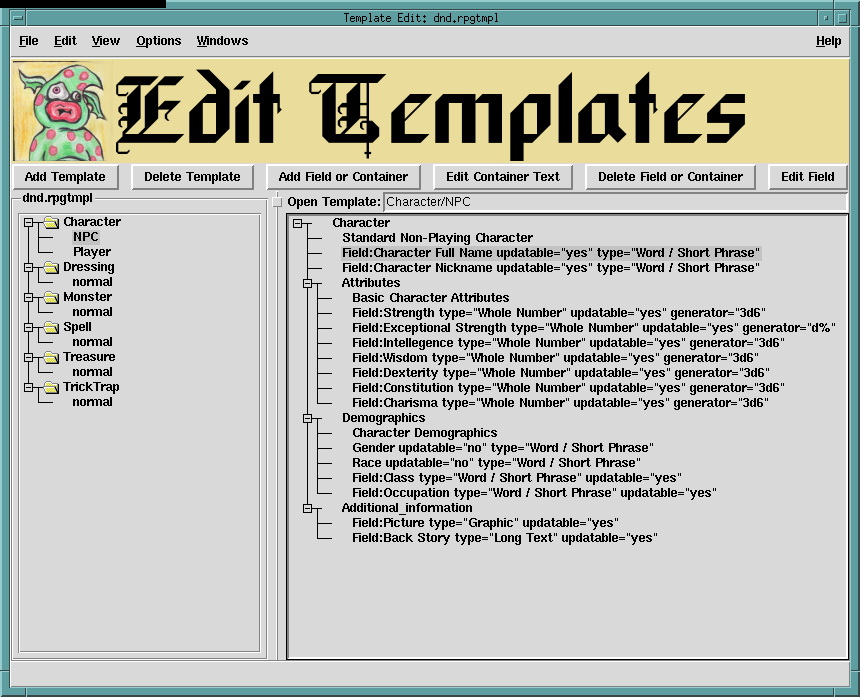
\includegraphics[width=5in]{TemplateEditor2.png}
\caption{The Template Editor Window after loading a template}
\label{fig:tmped2}
\end{centering}
\end{figure}
To allow for differences in game systems, game data elements are
defined with the use of templates.  These templates define what
information is recorded for each game element for a given game system. 
These templates are created and maintained with the template editor. 
The template editor in invoked from the Options menu.  The editor is
shown in Figures~\ref{fig:tmped1} and \ref{fig:tmped2}.  A sheet
contains a top level container which in turn contains zero or more fields
or containers.  Containers can contains zero or more fields or
containers.  Fields and containers have names. Fields also have a type,
possibly a generator (dice combination), and a flag that indicates whether the
field value can be updated.  There are five defined field types:

\index{Field types|(}
\begin{enumerate}
\item \verb=Whole Number=--This is a numerically valued field. It is either
an arbitrary (usually fixed) value or the result of a dice throw.
\item \verb=Word / Short Phrase=--This either a single word or a short
(one line at most) phrase, generally describing a textual attribute,
such as a name or some sort of descriptive condition or status.
\item \verb=Long Text=--This is a multi-line, but short (1-2 paragraph)
text value.
\item \verb=Graphic=--This is a picture file.  Most standard graphics
formats are supported, including GIF, PNG, JPEG, BMP, TIFF, TGA,
PostScript, and Sun Raster.  The graphic file will be displayed in the
sheet editor window.
\item \verb=Document=--This a document file.  Any sort of external file
is supported.  The external file will be copied into the sheet file. 
The sheet editor will not attempt to display or otherwise process the
file, but since the file will be ``carried'' along with the sheet file,
it will be available and extractable as needed.
\end{enumerate}
\index{Field types|)}

The generator attribute is only used for numerically valued fields and
the updatable attribute can only be set to no for the word / short
phrase and numerically valued fields.

The templates are used for Character, Monster, Spell, Treasure, Trick /
Trap, and Dressing sheet editors.  The Map editor uses a set of hard-coded
templates. These templates define the fields, their attributes, and
grouping / organizational structure.  Containers have a text attribute
that is used as a section heading for the group of fields contained in
the container. The included template file, \verb=dnd.rpgtmpl=, defines
informational sheets suitable for \textit{Advanced Dungeons and
Dragons}, but template files for other game systems can be created.

A template file is a Zip archive file containing directories for each
class of sheet: Character, Monster, Spell, Treasure, Trick / Trap, and
Dressing.  These directories in turn contain the template XML files,
which define the structure of the sheets.  It is possible to have
multiple templates for any given class.  It is also possible to have no
templates for a given class.  Not all game systems have all classes of
these things and others might have several sub-classes, sometimes with
very different attributes.

\section{Sheet Editor Windows}
\label{SheetEditor}

\begin{figure}[hbpt]
\begin{centering}
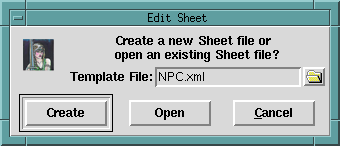
\includegraphics[width=5in]{CreateOrOpenChar.png}
\caption{The Open or Create Character dialog box}
\label{fig:opencreatechar}
\end{centering}
\end{figure}
\begin{figure}[hbpt] 
\begin{centering}
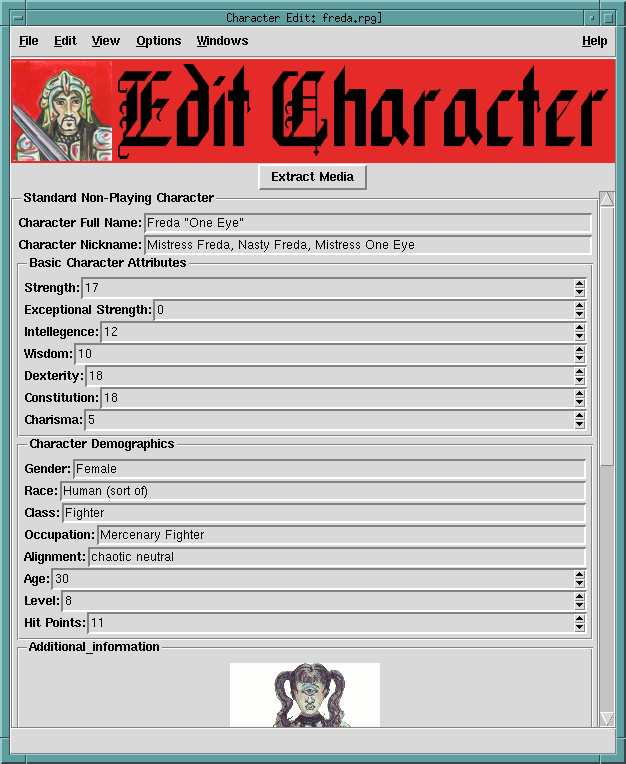
\includegraphics[width=5in]{CharacterEditor.png} 
\caption{The Character Editor window of the Role Playing Database} 
\label{fig:char}
\end{centering} 
\end{figure} 
The Sheet Editor Window, which includes the Character Editor, shown in
Figure~\ref{fig:char}, is used to edit characters, both playing and
non-playing characters, monsters, spells, treasure, tricks / traps, and
dressing items.  It uses one of the sheet templates defined in the
current template file (see Section~\ref{sect:configuration}).  When one
of the sheet editor buttons on the main window are clicked on, a small
dialog box is displayed (shown in Figure~\ref{fig:opencreatechar}),
asking if you want create a new sheet file, using a selected template
or open an existing sheet file. The Monster, Spell, Treasure,  Trick /
Trap, and Dressing Editor Windows are the same as the Character Editor,
but use different templates.

In addition to the fields created from the sheet template, there is also
a tool bar button, labeled ``Extract Media''.  This button allows for the
extraction of embedded media files contained within the sheet file. 
This allows for the use of external editors or viewers with these files.

A sheet file is a Zip archive containing two directories, xml and media.
The xml contains a file named sheet.xml, which is an XML file containing
the sheet information.  The media directory contains any media files
associated with the sheet--this could be pictures or other documents.

\section{Map Editing Window}
\label{Map}


